\documentclass[a4paper,12pt,twoside]{article}

%\usepackage{ucs}
\usepackage[utf8]{inputenc}
%\usepackage{babel}
%\usepackage{fontenc}
\usepackage[pdftex]{graphicx}

\usepackage[pdftex]{hyperref}

\author{Sara Gabrielli}
\title{Tutorial 2a exercise paper}
\date{09/14/17}

\begin{document}
 \maketitle
 
 \begin{center}
  \texttt{sa2743ga-s@lu.se}
 \end{center}

 \section{Introduction}
\label{sec:intro}

This is introduction. Summary is in Section \ref{sec:sum}

 \section{Protein structure}
\label{sec:prot struc}

\begin{figure}[h]
\begin{center}
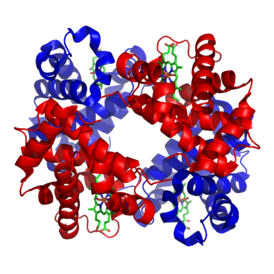
\includegraphics[width=4cm]{Haemo.png}
\caption{Structure of human hemoglobin}
\label{fig:hemo}
\end{center}
\end{figure}

Figure \ref{fig:hemo} shows the structure of a protein obtained by crystallography . For more details, check the Protein Data Bank~\cite{PDB}

\subsection{Levels of protein structure}
\label{sec:levels}

\begin{table}[h]
 \begin{center}
 \caption{List of the levels of protein structure}
 \label{types}
  \begin{tabular}{c|c} 
  \textbf{Level of structure}& \textbf{Description}\\ \hline \hline
  primary& sequence of the amino acids making up the protein chain\\ \hline
  secondary& regions of ordered structures in the protein chain \\ \hline
  tertiary& three-dimensional shape of the protein\\ \hline
  quaternary& held just by protein made up of subunits\\ \hline
  \end{tabular}

 \end{center}

\end{table}

Tabel \ref{types} lists the different levels of structure in a protein~\footnote{We can see from figure \ref{fig:hemo} that hemoglobin has a quaternary structure}

\section{About mathematics}
\label{sec:math}
$e^x$, $A_x$,$\lambda \cdot \rho \ldots $

\begin{equation}
 \sigma= \sqrt{ \frac{1}{N-1} \sum \limits_{i=1}^N (x_i-\mu)^2}
 \label{eq:std}
\end{equation}

\begin{equation}
\hat{H}~\Psi(r,t) = i \frac{h}{2\pi}\frac{\partial}{\partial{t}}~\Psi(r,t)
\label{eq:schrod}
\end{equation}

Equation \ref{eq:std} is the formula for the sample standard deviation.
Equation \ref{eq:schrod} is the time-dependent Schr\"odinger equation.

\section{Summary}
\label{sec:sum}
We learned the following:
\begin{itemize}
 \item Each protein has different levels of structure
 \item \LaTeX is good for:
 \begin{enumerate}
  \item Structuring very \textbf {good looking} documents
  \item Writing equations
 \end{enumerate}
 
 \begin{verbatim}
  \usepackage{verbatim}
 \end{verbatim}


\end{itemize}


\begin{thebibliography}{99}
 \bibitem{PDB} Protein Data Bank website: \url{https://www.rcsb.org/pdb/home/home.do}
\end{thebibliography}

 
 \end{document}
